\documentclass[11pt]{article}
\pagestyle{empty}
\usepackage{fancyhdr}
\usepackage{lastpage}
\usepackage{graphicx}
\graphicspath{ {images/} }
\pagestyle{fancy}
\renewcommand{\headrulewidth}{0pt}
\cfoot[R]{\thepage~of~\pageref{LastPage}}
\addtolength{\oddsidemargin}{-.875in}
\addtolength{\evensidemargin}{-.875in}
\addtolength{\textwidth}{1.75in}
\addtolength{\topmargin}{-.875in}
\addtolength{\textheight}{1.75in}

\begin{document}
\begin{center}
\textbf{Database Systems Homework 2}
\end{center}

We are required to produce a Crow's feet diagram from the following ER diagram:
\begin{center}
    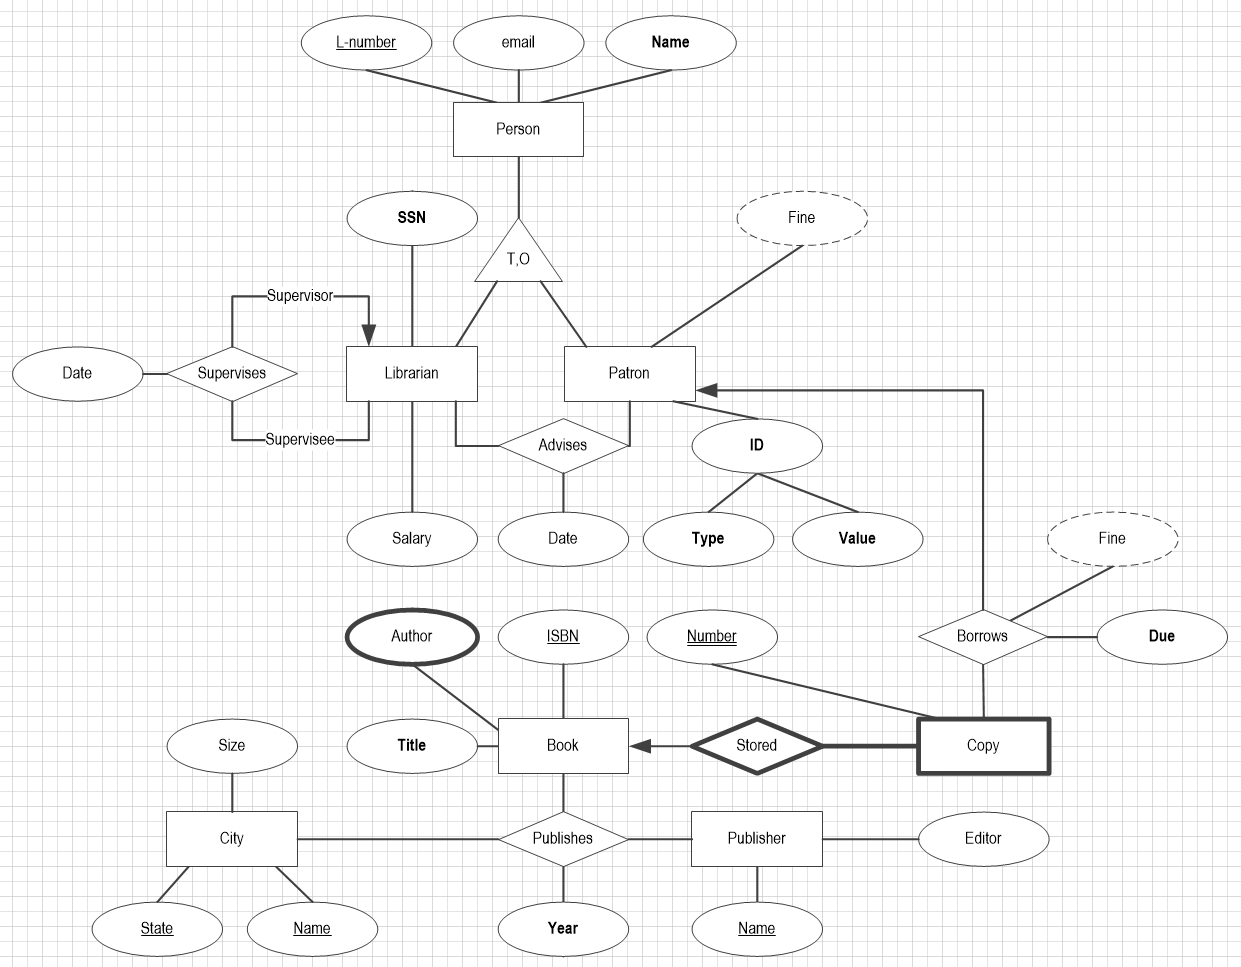
\includegraphics[width=180mm]{problem.jpg}
\end{center}
The ER diagram also contains the following annotations on a second page:
\begin{itemize}
    \item A \textbf{Patron} must \textbf{Borrow} at least one \textbf{Copy} from the library
    \item For a \textbf{Librarian}, \textbf{SSN} is never Null
    \item For a \textbf{Patron}, \textbf{Type} and \textbf{Value} are never Null and no two patrons can have the same tuple (\textbf{Type}, \textbf{Value})
    \item \textbf{Date} in \textbf{Advises} is never Null
    \item \textbf{Due} in \textbf{Borrows} is never Null
    \item \textbf{Fine} in \textbf{Borrows} is calculated if the book is overdue i.e. if Current Date $<$ Due Date then \textbf{Fine} = (Due Date - Current Date)*2, otherwise it is Null
    \item \textbf{Fine} in \textbf{Patron} is the sum of the fines on books patron has borrowed and not yet returned
\end{itemize}
\begin{center}
    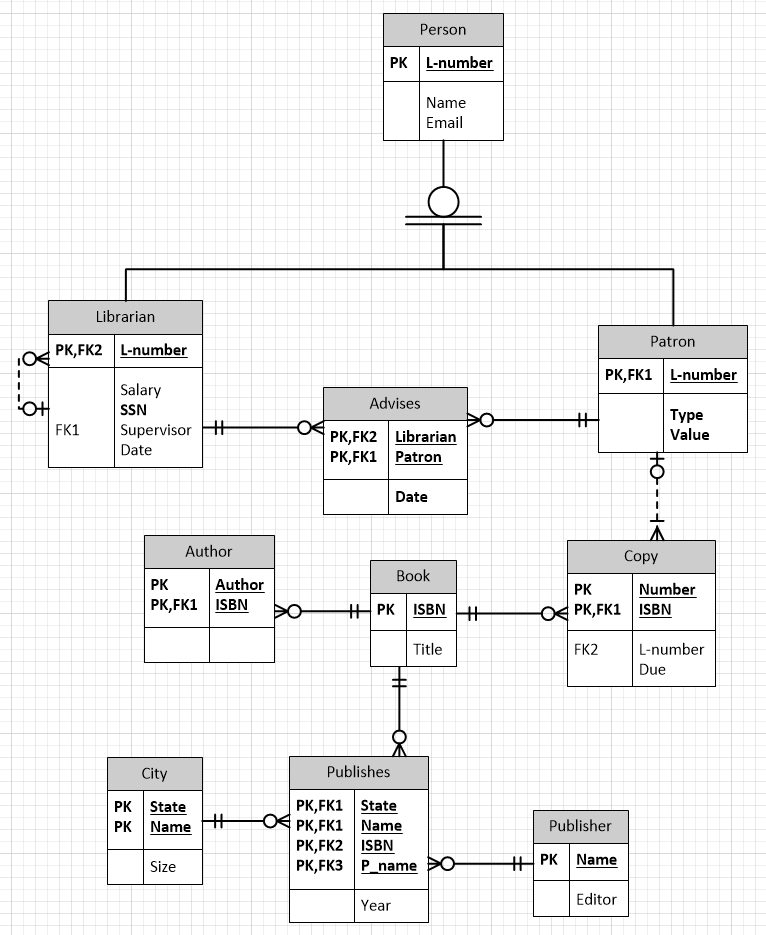
\includegraphics[width=150mm]{solution.jpg}
\end{center}
The Crow's feet annotation diagram also contains the following annotations on a second page:
\begin{itemize}
    \item In \textbf{Patron}, (\textbf{Type}, \textbf{Value}) is UNIQUE
    \item \textbf{Fine} in \textbf{Borrows} is calculated if the book is overdue i.e. if Current Date $<$ Due Date then \textbf{Fine} = (Due Date - Current Date)*2, otherwise it is Null
    \item \textbf{Fine} in \textbf{Patron} is the sum of the fines on books patron has borrowed and not yet returned
    \item In \textbf{Copy}, \textbf{L-number} and \textbf{Due} are either both Null or not Null. A copy of book can either be borrowed or not borrowed.
\end{itemize}

\end{document}